We evaluate the main test split of the SpinGlassBench benchmark at $n=24$: Gaussian SK instances, seven inverse temperatures $\beta\in\{0.3,0.6,0.9,1,1.2,1.5,2\}$, an equal budget of $10^5$ energy evaluations per estimate across all methods, exact $\log Z$ from Gray-code enumeration, and 5 seeds per instance. Classical estimators were evaluated across $\vinstClassical$ instances ($1{,}000$ runs total); computationally intensive learned methods were trained and evaluated across $\vinstLearnedMin$ to $\vinstLearnedMax$ instances ($100$ to $150$ runs total). Table~\ref{tab:chemical_audit} and Figure~\ref{fig:audit_comparison} report summary metrics from this benchmark.

\begin{table}[t]
\centering\small
\caption{SK, $n=24$, test split, $10^5$ energy evaluations per estimate, 5 seeds per instance. Error: mean $|\log\hat Z-\log Z|/n$. Coverage: share of nominal 95\% intervals containing exact $\log Z$ (Clopper-Pearson 95\% binomial CIs in text); n/a: method reports no interval. Seconds: mean wall-clock per estimate at $\beta=1.5$, one thread; learned methods include training.}
\label{tab:chemical_audit}
\begin{tabular}{lrrrrr}
\toprule
Method & \multicolumn{2}{c}{$|\log\hat Z-\log Z|/n$} & \multicolumn{2}{c}{Coverage (\%)} & Seconds \\
\cmidrule(lr){2-3}\cmidrule(lr){4-5}
 & $\beta=0.6$ & $\beta=1.5$ & $\beta=0.6$ & $\beta=1.5$ & per estimate \\
\midrule
SA-TI & $2.4\times10^{-4}$ & $7.1\times10^{-4}$ & n/a & n/a & 0.06 \\
PT-TI & $2.8\times10^{-4}$ & $8.7\times10^{-4}$ & n/a & n/a & 0.11 \\
AIS & $2.7\times10^{-4}$ & $8.9\times10^{-4}$ & 96 & 94 & 0.07 \\
SMC & $2.7\times10^{-4}$ & $8.8\times10^{-4}$ & 96 & 95 & 0.07 \\
PA & $2.7\times10^{-4}$ & $7.8\times10^{-4}$ & 96 & 96 & 0.08 \\
\midrule
VAN-MADE & $2.7\times10^{-5}$ & $8.6\times10^{-5}$ & 95 & 96 & 2.49 \\
Masked diffusion & $1.6\times10^{-4}$ & $1.3\times10^{-2}$ & 94 & 60 & 6.96 \\
GFlowNet & $1.5\times10^{-3}$ & $2.4\times10^{-2}$ & 94 & 71 & 30.60 \\
\bottomrule
\end{tabular}

\end{table}

\begin{figure}[t]
\centering
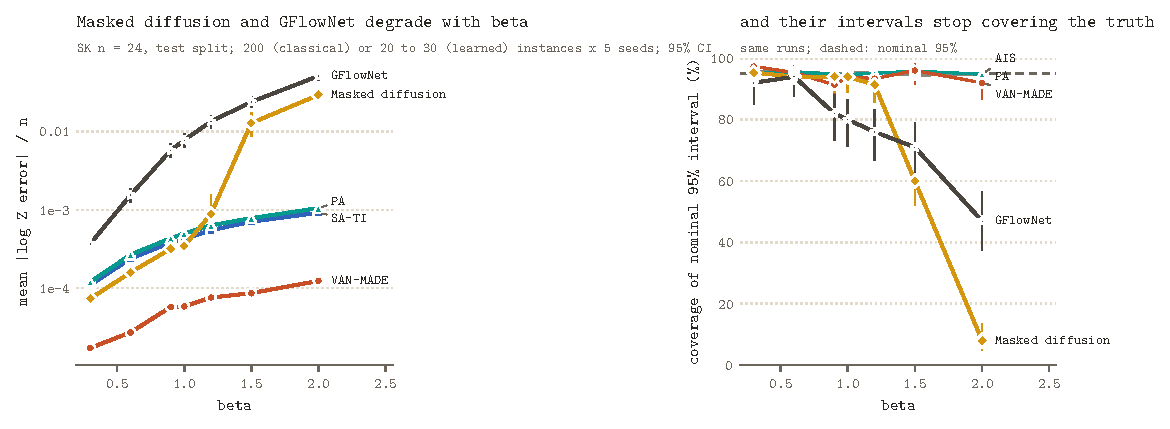
\includegraphics[width=\linewidth]{figures/fig_audit_comparison.pdf}
\caption{Left: mean absolute error of $\log Z$ per spin against $\beta$. Right: coverage of nominal 95\% intervals. SK $n=24$, test split, 5 seeds per instance; error bars are 95\% intervals over instances. Dashed: nominal 95\%.}
\label{fig:audit_comparison}
\end{figure}

\paragraph{Accuracy and architectural divergence.} At $\beta=1.5$, error per spin is $\verrSATIOneFive$ for simulated annealing with thermodynamic integration (SA-TI) and $\verrPAOneFive$ for population annealing (PA). Crucially, learned samplers show sharp architectural divergence:
\begin{itemize}
\item \textbf{Normalized autoregressive networks (VAN-MADE):} Achieve the highest accuracy per energy evaluation ($\verrVANOneFive$, roughly $\vvanOverSati$ times lower error than SA-TI) and maintain calibrated coverage across all temperatures: $\vcovVANZeroSix\%$ at $\beta=0.6$ ($\vcovNVANZeroSix$ runs; 95\% Clopper-Pearson interval $\vcovCIVANZeroSix$), $\vcovVANOneFive\%$ at $\beta=1.5$ ($\vcovCIVANOneFive$), and $\vcovVANTwo\%$ at $\beta=2$ ($\vcovCIVANTwo$), close to PA at $\beta=2$ ($\vcovPATwo\%$, $\vcovNPATwo$ runs, $\vcovCIPATwo$). A possible reason, which we have not tested, is that an autoregressive model's exactly normalized probabilities make the reverse-KL gradient sensitive to missing mass. However, this relies on a 1D sequence factorization ($p(\sigma)=\prod_i p(\sigma_i\mid\sigma_{<i})$). In continuous 3D molecular coordinates, autoregressive factorizations over all atom positions are geometrically constrained and break Euclidean equivariance, which is one reason diffusion models and continuous flows are more common in chemistry.
\item \textbf{Iterative generative samplers (Masked Diffusion and GFlowNets):} Are one to two orders of magnitude less accurate ($\verrDiffOneFive$ and $\verrGFNOneFive$) and undergo catastrophic calibration collapse in the spin-glass phase ($\beta \ge 1.5$). Masked diffusion coverage falls from $\vcovDiffZeroSix\%$ ($\vcovCIDiffZeroSix$) at $\beta=0.6$ to $\vcovDiffOneFive\%$ ($\vcovCIDiffOneFive$) at $\beta=1.5$ and $\vcovDiffTwo\%$ ($\vcovNDiffTwo$ runs, $\vcovCIDiffTwo$) at $\beta=2$. GFlowNet coverage drops to $\vcovGFNOneFive\%$ ($\vcovCIGFNOneFive$) and $\vcovGFNTwo\%$ ($\vcovNGFNTwo$ runs, $\vcovCIGFNTwo$).
\end{itemize}
On one test instance, illustrated in the companion paper, the diffusion sampler keeps one side of the overlap distribution and the GFlowNet concentrates on a few overlaps. By Proposition~\ref{prop:unvisited}, this omitted mass does not widen nominal intervals, producing false confidence.

\paragraph{Wall-clock trade-offs.} Table~\ref{tab:chemical_audit} reports single-thread CPU execution time, with learned methods including training. Under this metric, SA-TI finishes in $\vsecSATI$\,s and PA in $\vsecPA$\,s, whereas VAN-MADE requires $\vsecVAN$\,s and diffusion requires $\vsecDiff$\,s. While neural samplers can amortize training costs when millions of samples are required, on single-target free-energy evaluations classical annealing remains substantially faster.

\paragraph{External code audits.} The companion SpinGlassBench study used the same exact references to score released checkpoints of published samplers; we summarize its results. In MDNS \citep{zhu2025mdns}, the released free-energy estimator rounds one per-step term in bfloat16, which biases $\log Z$ upward by up to $4.6\times10^{-4}$ per site; a one-line change removes the bias. MetaDNS \citep{du2026metadns}, which shares this code, is unbiased at its float16 default. In LEAPS \citep{holderrieth2025leaps}, free energies at the released time grids are low by $2.2$ to $3.2\times10^{-3}$ per site, mostly from time discretization. The ESS did not reveal these errors: for MDNS the biased and corrected estimators have nearly the same ESS, and for LEAPS the ESS fraction is 0.82 on Ising (biased) and 0.31 on Potts, where it is no higher at the finer grids that reduce the bias.